\section{Resultados globales}

\begin{figure}[ht]
    \centerfloat
    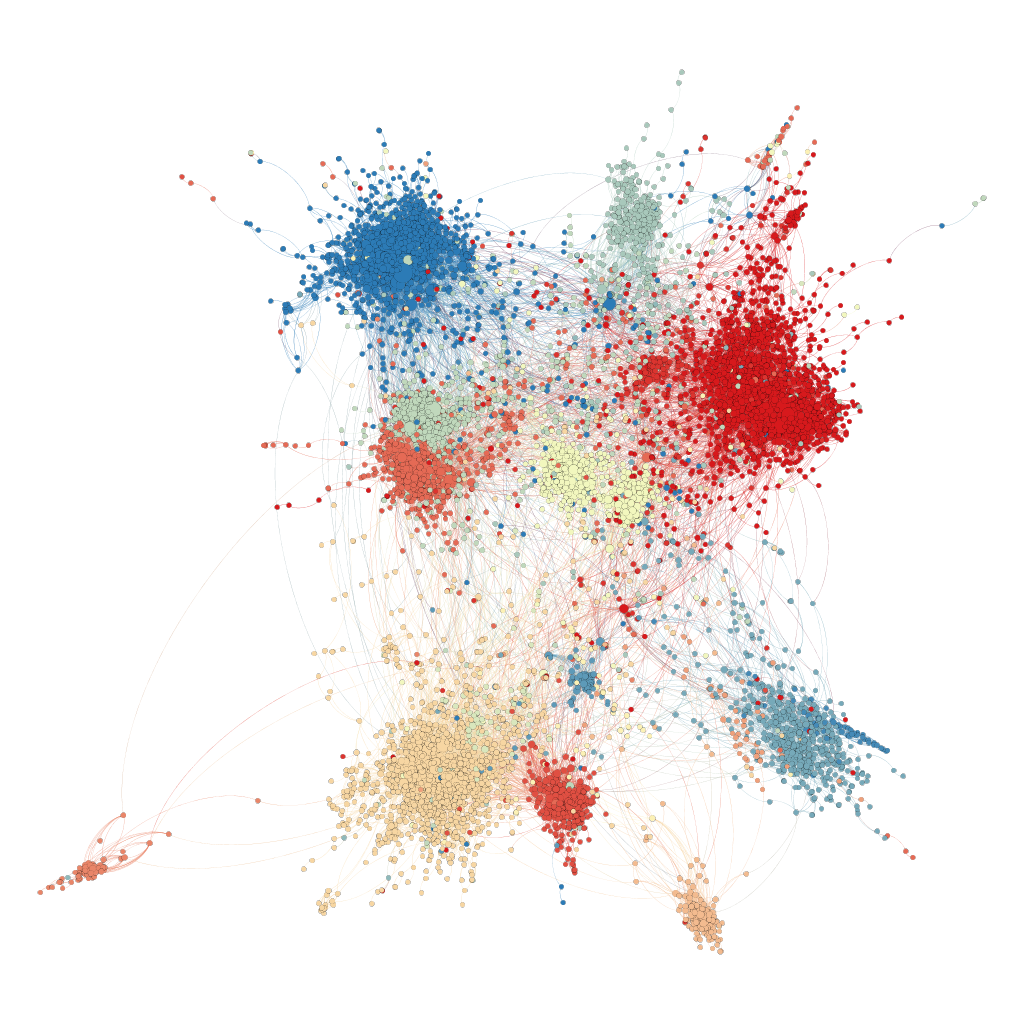
\includegraphics[width=1.097\textwidth]{img/resultados/grado-targets.png}
    \caption{Topología de la red. El color indica el país de cada usuario.}
\end{figure}

\begin{figure}[t]
    \centering
    \resizebox{0.78\columnwidth}{!}{%
    \begin{tabular}{| l | r |} 
        \hline
        \textbf{Medida} & \textbf{Valor} \\
        \Xhline{2\arrayrulewidth}
        Número de nodos \textbf{N} & 7,624 \\
        \hline
        Número de enlaces \textbf{L}	& 27,806 \\
        \hline
        Número máximo de enlaces \textbf{$L_{max}$} & 58117752 \\
        \hline
        Densidad del grafo \textbf{$L/L_{max}$} & 0.001 \\
        \Xhline{2\arrayrulewidth}
        Grado medio \textbf{<k>} & 7.294 \\
        \hline
        Diámetro \textbf{$d_{max}$} & 15 \\
        \hline
        Distancia media \textbf{d} & 5.232237269 \\
        \hline
        Coeficiente medio de clustering \textbf{<C>} & 0.285 \\
        \Xhline{2\arrayrulewidth}
        Número de componentes conexas & 1 \\
        \hline
        Número de nodos componente gigante (y \%) & 7,624 (100) \\
        \hline
        Número de aristas componente gigante (y \%) & 27,806 (100) \\
        \hline
    \end{tabular}
    }
    \caption{Medidas globales de la red.}
\end{figure}

\begin{figure}[ht]
    \centerfloat
    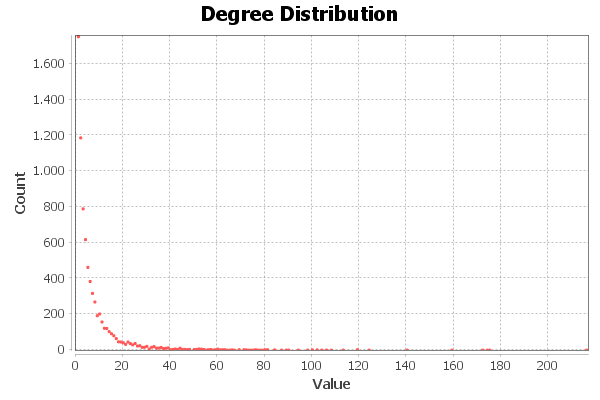
\includegraphics[width=0.9\textwidth]{img/resultados/gradoMedio/degree-distribution.png}
    \caption{Distribución de grados.}
\end{figure}

\begin{figure}[ht]
    \centerfloat
    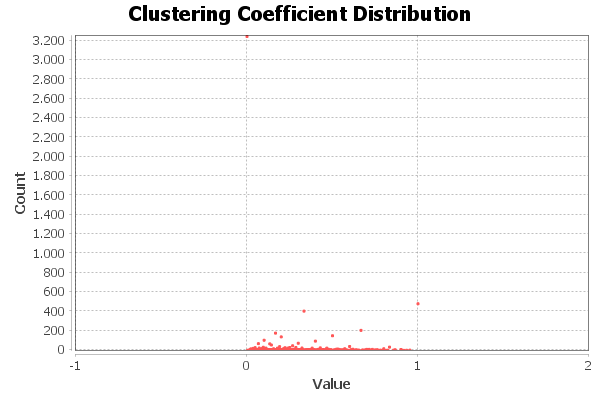
\includegraphics[width=0.9\textwidth]{img/resultados/clusteringMedio/clustering-coefficient.png}
    \caption{Distribución del clustering medio de la red.}
\end{figure}

\begin{figure}[ht]
    \centerfloat
    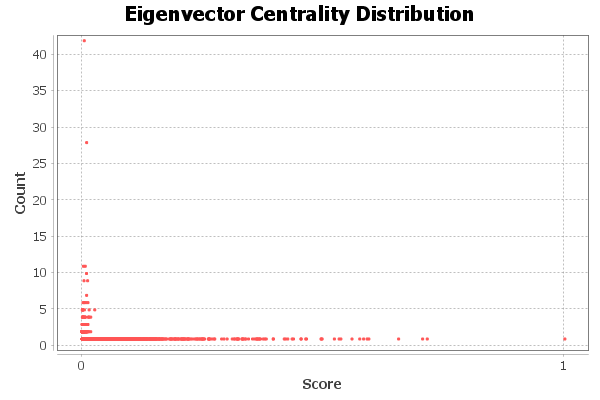
\includegraphics[width=0.9\textwidth]{img/resultados/vectorPropio/eigenvector-centralities.png}
    \caption{Distribución de los valores de vector propio.}
\end{figure}